\documentclass{beamer}

\usepackage[ngerman]{babel}
\usepackage[utf8]{inputenc}
\usepackage{hyperref}
\usepackage{eurosym}

\mode<presentation>{
	\definecolor{LogoRed}{RGB}{219,00,31}
	\definecolor{LogoGray}{RGB}{86,86,80}
	
	\useoutertheme[width=2.1cm]{sidebar}
	\useinnertheme{rounded}
	\setbeamercolor{normal text}{fg=black,bg=white}
	\setbeamercolor{palette sidebar primary}{use=normal text,fg=normal text.fg}
	\setbeamercolor{title}{fg=LogoRed}
	\setbeamercolor{frametitle}{fg=LogoRed}
	\setbeamercolor{structure}{fg=LogoRed}
	\setbeamercolor{section in sidebar}{fg=LogoRed}
	\setbeamercolor{subsection in sidebar}{fg=LogoRed}
	
	\usefoottemplate{\vbox{\tinycolouredline{LogoGray!25}{\hspace{4pt}\hspace{15pt}\insertdate\hfill\insertshortinstitute\hfill \insertframenumber{}/\inserttotalframenumber}}}
	
	\setbeamertemplate{section in toc}{\inserttocsectionnumber.~\inserttocsection\par}
	\setbeamertemplate{subsection in toc}{\hspace*{2em}\inserttocsectionnumber.\inserttocsubsectionnumber~\inserttocsubsection}
	\AtBeginSubsection[] {
		\begin{frame}<beamer>
			\frametitle{Outline}
			\tableofcontents[currentsection,sectionstyle=show/show,subsectionstyle=show/shaded/hide]
		\end{frame}
	}
}

\title{Man-in-the-Middle-Angriffe}
\subtitle{Praktikum Datenschutz und Datensicherheit \\ Sommersemester 2016}
\author[Fabian Uhlmann \and{Diana Irmscher}]{Fabian Uhlmann
\and {Diana Irmscher}}
\institute[Hochschule für angewandte Wissenschaften München]{Fakultät für Informatik und Mathematik
\and{Hochschule für angewandte Wissenschaften München}}
\logo{
\includegraphics[height=1.0cm]{logo_hm.png}}
\date{\today}

\setbeamertemplate{navigation symbols}{}

\begin{document}
	\maketitle
	
	\section{Begrüßung}
	
	\begin{frame} %% Die Vortragenden stellen sich vor
		\frametitle{Vorstellung}
		\begin{columns}
			\column{.47\textwidth}
			
\includegraphics[width=0.7\textwidth]{uhlmann.jpg}\\
			\textbf{Fabian Uhlmann}
			\\
			Informatik, Bachelor
			\column{.47\textwidth}
			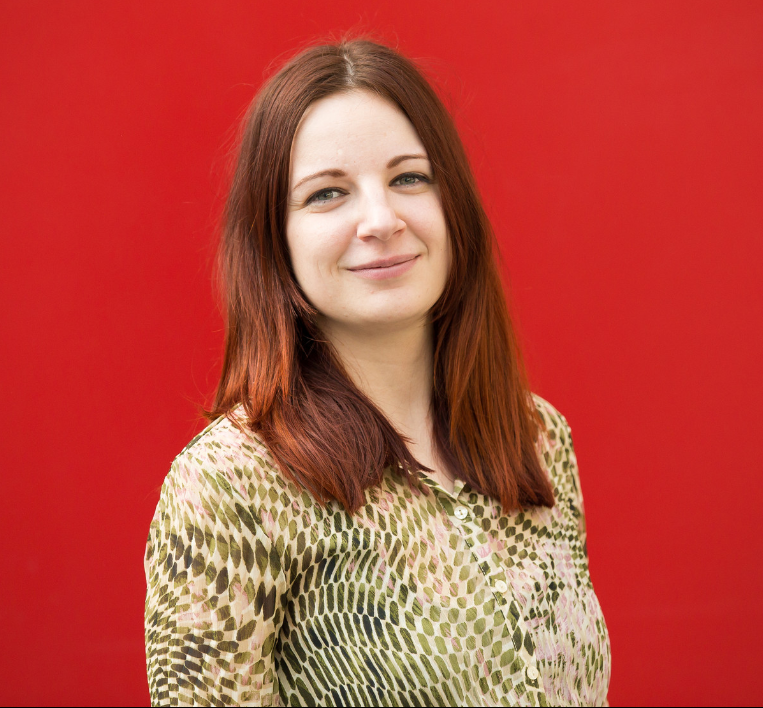
\includegraphics[width=0.725\textwidth]{irmscher.png}\\
			\textbf{Diana Irmscher}
			\\
			Informatik, Bachelor
		\end{columns}
		
		
		

	\end{frame}
	
	\begin{frame} %% Agenda zeigen, was noch ansteht
		\frametitle{Agenda}
		\tableofcontents
	\end{frame}
	
	\section{Man in the Middle im Web}
	
		\begin{frame}
			\frametitle{Aufgabenstellung}
			Dell und Lenovo haben demonstriert, dass man mit Man-in-the-Middle
			Angriffen die Sicherheit eines Systems sehr effizient aushebeln kann.
			Wie funktioniert ein derartiger Angriff und was kann man tun, um sich
			zu schützen.
	    \end{frame}
	     \subsection*{Einführung}
	     \begin{frame}
	     	\frametitle{Man in the Middle (MITM)}
	     	\begin{minipage}[t]{0.8\linewidth}
	     		%	\centering
	     		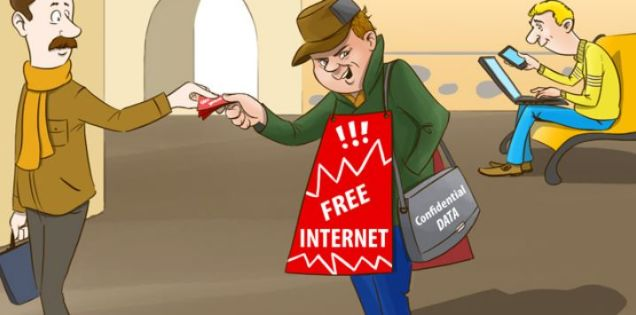
\includegraphics[width=0.8\linewidth]{images_fabian/mitm.jpg}
	     		\newline Quelle: [1]
	     	\end{minipage}% <- sonst wird hier ein Leerzeichen eingefügt
	     	\hfill
	     	\begin{minipage}[t]{0.7\linewidth}
	     	%	\centering
	     		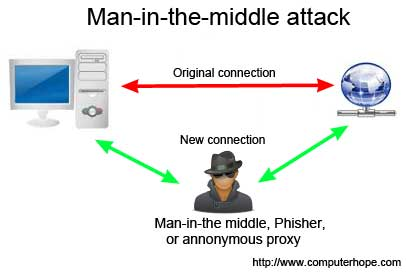
\includegraphics[width=0.8\linewidth]{images_fabian/mitm2.jpg}
	     		\newline Quelle: [2]
	     	\end{minipage}
	     \end{frame}
	     \begin{frame}
	     	\frametitle{HTTP(s) und Zertifikate}
	     	
	     \end{frame}
    
    \section{Man-in-the-Middle-Angriffe im geswitchten Netzwerk}
    	
    	\begin{frame}
    		\frametitle{Aufgabenstellung}
    		Es gibt Man-in-the-Middle-Angriffe nicht nur gegen SSL/TLS-Verbindungen, sondern auch gegen "normale" Netzwerkverbindungen. Sie werden von Angreifern eingesetzt, um in einem geswitchten Netz zu sniffen.
        \end{frame}
        \subsection*{Einführung}
        \begin{frame}
        	\frametitle{Hub}
            \begin{itemize}
            \item stellt Verbindungskomponente in einem Netzwerk dar
            \item arbeitet auf Schicht 1 des ISO-/OSI-Schichtenmodells
            \item nicht zielorientiert
            \item sendet Bits an alle Teilnehmer, die an Hub angeschlossen sind
            \item wurde in Netzwerken hauptsächlich aus Kostengründen eingesetzt
            \item wurde mittlerweile fast vollständig von Switches verdrängt, da diese mittlerweile günstig geworden sind 
            \end{itemize}
        \end{frame}
        
        \begin{frame}
          	\frametitle{Switch}
            	\begin{itemize}
            	\item arbeite auf Schicht 2 des ISO-/OSI-Schichtenmodell
            	\item zwei Typen:
            	\begin{itemize}
            	\item einfacher Switch : leitet Pakete mit Hilfe von MAC-Adressen von Quelle zu Ziel weiter; verwendet dafür Switch-Tabelle
            	\item Layer-3-Switch : zusätzlich zur oben genannten Funktion noch Überwachungsfunktionen möglich, z.B. IP-Filterung, Routing (Schicht 3)
            	\end{itemize}
            	\end{itemize}
            	Einsatz eines Switchtes bringt wesentliche Vorteile zum Vorgänger Hub
            	\begin{itemize}
            		\item erhöhte Datensicherheit
            		\item geringere Netzwerklast	
            	\end{itemize}
        \end{frame}
        
        \begin{frame}
        	\frametitle{Funktion Switch-Tabelle}
        	Switch-Tabelle ermöglicht wesentlichen Punkt der Funktionsweise:
        	\begin{itemize}
        	\item Switch verfügt über Ein- und Ausgänge, sogenannte Ports
        	\item können unabhängig voneinander empfangen und senden
        	\item an Ein- und Ausgängen sind einzelne Netzwerkteilnehmer angeschlossen
        	\item für jeden Port MAC-Adresse des Teilnehmers hinterlegt
        	\end{itemize}  	
    	\end{frame}
    	
    	\begin{frame}
	       	\frametitle{Funktion Switch-Tabelle}
	       	Store-und-Forward-Prinzip
	       	\begin{enumerate}
	       	\item Switch empfängt gesamtes Frame, berechnet CRC, wenn CRC nicht stimmt, wird Frame verworfen
	       	\item überprüfen, ob Quell-Adresse in Switch-Tabelle, wenn nicht, Eintrag zusammen mit Port in Switch-Tabelle
	       	\item Ziel-Adresse mit Einträgen in Switch-Tabelle vergleichen, wenn vorhanden, wird an Teilnehmer mit passenden Port weitergeleitet, ansonsten Weiterleitung an alle Ports
	       	\end{enumerate}  	
	   	\end{frame}
    	
        \begin{frame}
        	\frametitle{Was ist ein geswitchtes Netzwerk}
        	\begin{itemize}
        	\item Auslastung des Netzwerkes stark reduziert
        	\item Frame nur noch an einen Teilnehmer, wenn dieser bekannt
        	\item Switch kann Teilnehmer auch in Gruppen aufspalten und unterscheiden, an welche Gruppe Frame gesendet wird
        	\item nahezu jeden Netzwerk verfügt heute über mindestens einen Switch
        	\end{itemize} 	
    	\end{frame}
    	
    	\begin{frame}
	       	\frametitle{Mehrere Switches in einem Netzwerk}
	       	\begin{itemize}
	       	\item natürlich möglich
	       	\item kann man nicht einfach miteinander verbinden, da sonst eine Schleife gelegt wird, gesamter Netzwerkverkehr kommt zum Erliegen
	       	\item Vorkehrungen treffen, spezielle Kabel
	       	\end{itemize} 	
	   	\end{frame}
    	
    	\subsection*{Angriffsmöglichkeiten}
        \begin{frame}
        	\frametitle{Angriffsmöglichkeiten}
        	
        	\begin{itemize}
 
        	\item MAC-Flooding
  
        	\item MAC-Spoofing

        	\item ARP-Spoofing
        	\end{itemize}
                       	
    	\end{frame}
    	
        \begin{frame}
        	\frametitle{MAC-Flooding}
        	\begin{itemize}
	       	\item Speicher in Switch-Tabelle ist begrenzt
	       	\item Switch wird mit gefälschten MAC-Adressen überhäuft, bis Speicher in der Tabelle voll
	       	\item wenn Tabelle voll, verhält sich Switch bei neuen Adressen wie Hub, weil diese unbekannt sind
	       	\item einige Switches haben Schutzmaßnahmen dagegen, z.B. List mit zugelassenen Ports anlegen
	       	\end{itemize} 
                       	
    	\end{frame}
		\begin{frame}
        	\frametitle{MAC-Spoofing}
        	\begin{itemize}
        	\item Quell-Adresse mit Adresse des Angreifers ersetzen
        	\item Antwort des Empfängers wird an Angreifer gesendet
        	\item Angreifer wird dabei allerdings in Switch-Tabelle eingetragen
        	\item Schutzmaßnahme: Liste mit erlaubten MAC-Adresse für jeweiligen Port
        	\end{itemize}
                       	
    	\end{frame}
    	\begin{frame}
    		\frametitle{ARP-Spoofing}
    		Dieser Angriff macht sich Schwachstelle des ARP-Protokolls zunutze.\\
    		Funktionsweise ARP:
    		\begin{itemize}
    		\item Auflösung IP zu Hardware-Adresse
    		\item jeder Rechner hat ARP-Tabelle
    		\item in ARP-Tabelle alle bekannten Teilnehmer des lokalen Netzwerkes hinterlegt
    		\item damit Einträge nicht veralten, regelmäßig ARP-Request
    		\end{itemize}  	
    	\end{frame}
    	
    	\begin{frame}
    		\frametitle{ARP-Schwächen im Protokoll}
    		\begin{itemize}
    		\item jede ARP-Response wird ausgewertet, auch ohne ARP-Request
    		\item Identität des Teilnehmers wird nicht überprüft
    		\end{itemize}           	
    	\end{frame}
    	
    	\begin{frame}
	   		\frametitle{ARP-Beispiel}
	   		Netzwerkteilnehmer
	   		\begin{itemize}
	   		\item Diana
	   		\item Fabian
	   		\item X
	   		\item Y Angreifer
	   		\end{itemize}           	
	   	\end{frame}
	   	
	   	\begin{frame}
	   		\frametitle{ARP-Beispiel}
	   		APR-Tabellen-Einträge mit entsprechenden Werkzeugen manipulieren, sodass in bei den Netzwerkteilnehmern falsche Angaben hinterlegt sind
	   			\vfill
			   	\begin{tabular}{l c l}
			   		ARP-Tabelle von Fabian & & \\
			   		\hline
			   		IP-Adresse Diana & : & MAC-Adresse von Y \\
			   		IP-Adresse X & : & MAC-Adresse von X \\
			   		IP-Adresse Y & : & MAC-Adresse von Y \\
			   	\end{tabular}
			   	\vfill
			   	\begin{tabular}{l c l}
			   		ARP-Tabelle von Diana & & \\
			   		\hline
			   		IP-Adresse Fabian & : & MAC-Adresse von Y \\
			   		IP-Adresse X & : & MAC-Adresse von X \\
			   		IP-Adresse Y & : & MAC-Adresse von Y \\
			   	\end{tabular}         	
	   	\end{frame}
	   	
	   	\begin{frame}
	   		\frametitle{ARP-Beispiel}
	   		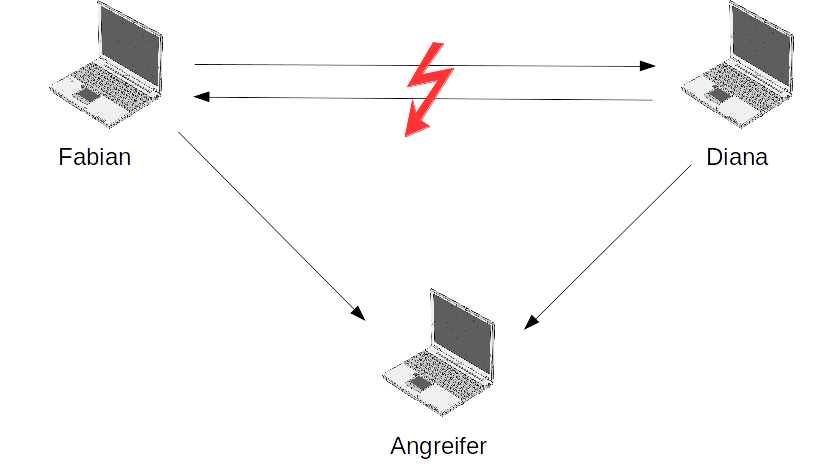
\includegraphics[height=5.0cm]{ARP-Tabelle-manipuliert.png}
	   	\end{frame}
	   	
	   	\begin{frame}
	   		\frametitle{ARP-Beispiel}
	   		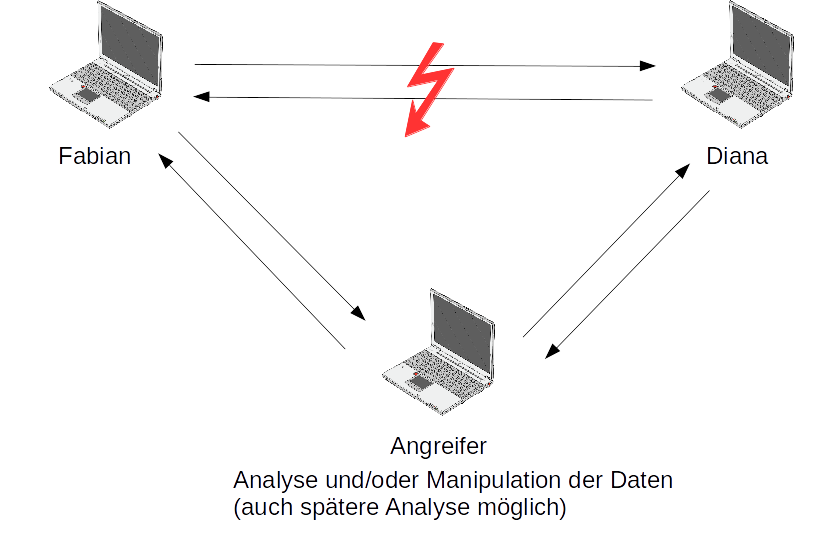
\includegraphics[height=5.0cm]{ARP-Tabelle-manipuliert_1.png}
	   	\end{frame}
    	
    	\subsection*{Werkzeuge}
		\begin{frame}
        	\frametitle{Werkzeuge}
                       	
    	\end{frame}
    	\subsection*{Maßnahmen}
		\begin{frame}
        	\frametitle{Schutzmaßnahmen}
                       	
    	\end{frame}

	\section{Literatur}
    	\begin{frame}
    		\frametitle{Literatur}
    		\addcontentsline{toc}{section}{Literatur}
    		\begin{enumerate}
    			\item http://hackerspace.kinja.com/how-to-defend-yourself-against-mitm-or-man-in-the-middl-1461796382
    			\item http://blog.agupieware.com/2013_10_01_archive.html
    		\end{enumerate}
    	\end{frame}    
\end{document}